\documentclass[12pt]{article}
\usepackage[a4paper, total={7in, 10in}]{geometry}
%\usepackage[utf8]{inputenc}
\usepackage{amsmath}
\usepackage{amsfonts}
\usepackage{amssymb}
\usepackage{amsthm}
\usepackage{caption}
\usepackage{subcaption}
\usepackage{xeCJK}
\usepackage{fontspec}
\usepackage{graphicx}
\usepackage{float}
\usepackage{hyperref}
\usepackage{bussproofs}
\usepackage{mathtools}
\usepackage{indentfirst}
\usepackage{xcolor}
\usepackage{listings}
\usepackage{afterpage}
\usepackage[backend=biber]{biblatex}

\theoremstyle{definition}
\newtheorem{theorem}{Theorem}[subsection]
\newtheorem{definition}[theorem]{Definition}
\newtheorem{corollary}{Corollary}[theorem]
\newtheorem{lemma}[theorem]{Lemma}
\newtheorem{proposition}[theorem]{Proposition}
\DeclareMathOperator{\trace}{\text{tr}}
\DeclareMathOperator{\diag}{\text{diag}}
\newcommand{\colvec}[2][0.8]{
  \scalebox{#1}{
    \renewcommand{\arraystretch}{.8}
    $\begin{bmatrix}#2\end{bmatrix}$
  }
}

\definecolor{backcolor}{rgb}{0.925,0.925,0.925}
\definecolor{codegray}{rgb}{0.5,0.5,0.5}
\definecolor{comment}{RGB}{85, 180, 85}
\definecolor{string}{RGB}{85, 85, 180}
\definecolor{keyword}{RGB}{220, 15, 220}


\lstdefinestyle{C}{
    language=C,
    basicstyle=\ttfamily\footnotesize,
    backgroundcolor=\color{backcolor},
    numberstyle=\tiny\color{codegray},
    commentstyle=\color{comment},
    stringstyle=\color{string},
    keywordstyle=\color{keyword},
    numbers=left,
    numbersep=5pt,
    breakatwhitespace=false,         
    breaklines=true,                 
    captionpos=b,                    
    keepspaces=true,                
    tabsize=4
}

\lstdefinestyle{C*}{
    language=C,
    basicstyle=\ttfamily\footnotesize,
    backgroundcolor=\color{backcolor},
    numberstyle=\tiny\color{codegray},
    commentstyle=\color{comment},
    stringstyle=\color{string},
    keywordstyle=\color{keyword},
    numbers=none,
    breakatwhitespace=false,         
    breaklines=true,                 
    captionpos=b,                    
    keepspaces=true,                
    tabsize=4
}

\lstdefinestyle{zsh}{
    language=bash,
    basicstyle=\ttfamily\footnotesize,
    backgroundcolor=\color{backcolor},
    numberstyle=\tiny\color{codegray},
    numbers=none,
    breakatwhitespace=false,         
    breaklines=true,                 
    captionpos=b,                    
    keepspaces=true,                
    tabsize=4
}

%%%%%%%%%%%%%%%%%%%%%%%%%%%%%%
\setCJKmainfont{Noto Sans CJK TC}
\setCJKmonofont{Noto Sans Mono CJK TC}
\setmainfont{Noto Serif Light}
\setsansfont{Noto Sans}
\setmonofont[Scale=MatchLowercase]{Noto Mono}
\renewcommand{\baselinestretch}{1.25}
\setlength{\parindent}{2em}
%%%%%%%%%%%%%%%%%%%%%%%%%%%%%%
\begin{filecontents}[overwrite]{\jobname.bib}
@misc{ncurses-howto,
  title = {NCURSES Programming HOWTO},
  author = {Padala, Pradeep},
  howpublished = {\url{https://tldp.org/HOWTO/NCURSES-Programming-HOWTO/}},
}
\end{filecontents}

\addbibresource{\jobname.bib}
\begin{document}
%%%%%%%%%%%%%%%%%%%%%%%%%%%%%%
\title{A Brief Introduction to ncurses\\
  \large 111-2 Programming(II) Bonus}
\author{Hsin-Yen, Chiang}
\maketitle
\tableofcontents
%%%%%%%%%%%%%%%%%%%%%%%%%%%%%%
\section{安裝與測試}
\noindent
在 Linux \footnote{\ 此處以 Ubuntu 22.04 為例} 下,我們執行以下指令:
\begin{lstlisting}[style=zsh]
  $ sudo apt-get install libncurses5-dev
\end{lstlisting}
在 macOS \footnote{\ 此處以 Ventura 13.0.1 為例} 下,我們執行以下指令:
\begin{lstlisting}[style=zsh]
  % brew install ncurses
\end{lstlisting}
即可完成安裝。此處使用的版本為 stable 6.4。我們使用以下程式測試 \texttt{ncurses} 是否已經被順利安裝。
\begin{lstlisting}[style=C]
  // test.c
  #include <ncurses.h>

  int main()
  {
      initscr();               // 初始化
      printw("Hello world!");  // 在螢幕上印出 Hello World!
      refresh();               // 更新視窗
      getch();                 // 等待使用者輸入
      endwin();                // 結束 curses 模式
      return 0;
  }
\end{lstlisting}

\noindent
我們在目錄 \texttt{40990131M\_BONUS} 下使用 \texttt{make} 指令 \footnote{\ 從此處開始,若沒有特別說明,則皆適用於本文所使用的 macOS 與 Linux 版本。}:
\begin{lstlisting}[style=zsh]
  % make
  gcc test.c -o test -lncurses
  ...
  Complete successfully.
\end{lstlisting}
注意我們需要使用 \texttt{-lncurses}。執行結果如下:
\begin{lstlisting}[style=zsh]
  % ./test
\end{lstlisting}
\begin{center}
    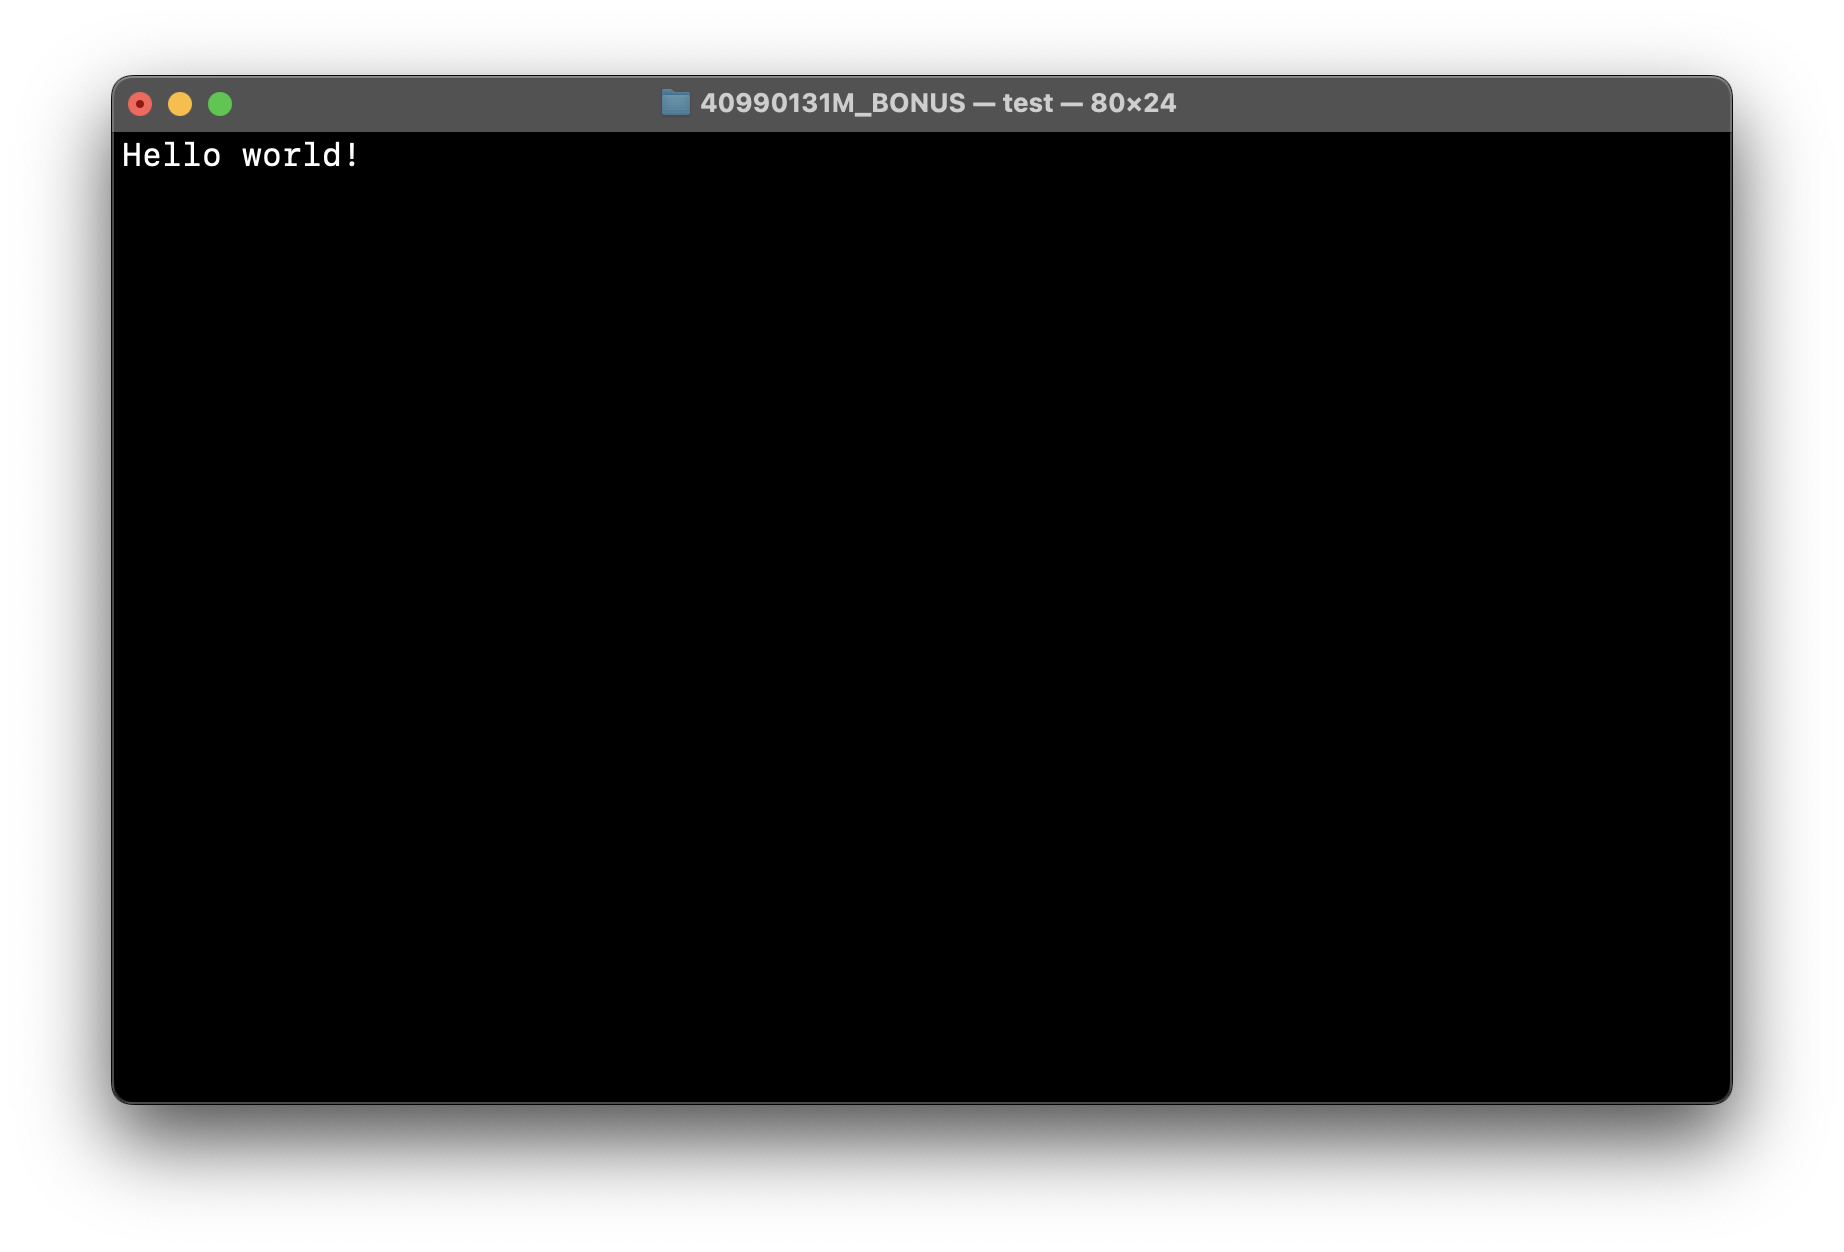
\includegraphics[width=\textwidth]{test.png}
\end{center}

\section{使用}
\noindent
接下來的章節將會粗略地介紹 \texttt{ncurses} 的功能。

\subsection{初始化}
\noindent
在我們呼叫完 \texttt{initscr()} 後,通常會呼叫一些初始化函式。其中,\texttt{raw()} 可以禁用 line buffering。函式 \texttt{noecho()} 可以禁用回顯 (echoing),這可以讓資訊的輸出更好掌控。函式 \texttt{keypad()} 可以讀取功能鍵。

\subsection{輸入與輸出}
\noindent
輸入與輸出各有三種對應的函式可供使用,如下表所示:
\begin{center}
    \begin{tabular}{|c|c|c|}
        \hline
        \textbf{輸出} & \textbf{輸入} & \textbf{描述} \\
        \hline\hline
        \texttt{addch()} & \texttt{getch()} & 輸出/輸入一個字符 \\
        \hline
        \texttt{printw()} & \texttt{scanw()} & 輸出/輸入 formatted string \\
        \hline
        \texttt{addstr()} & \texttt{getstr()} & 輸出/輸入字串 \\
        \hline
    \end{tabular}
\end{center}

\subsubsection{\texttt{addch()}}
\noindent
以下程式展示了 \texttt{addch()} 函式的使用方法:
\begin{lstlisting}[style=C]
  // addch.c
  #include <ncurses.h>

  int main()
  {
      initscr();
      raw();
      noecho();
    
      move(12, 40);  // Move cursor to row 12, column 40
      addch('*');    // Add the character '*' at the current cursor position
    
      refresh();
      getch();
      endwin();
      return 0;
  }
\end{lstlisting}

\newpage
\noindent
執行結果如下:
\begin{lstlisting}[style=zsh]
  % ./addch
\end{lstlisting}
\begin{center}
    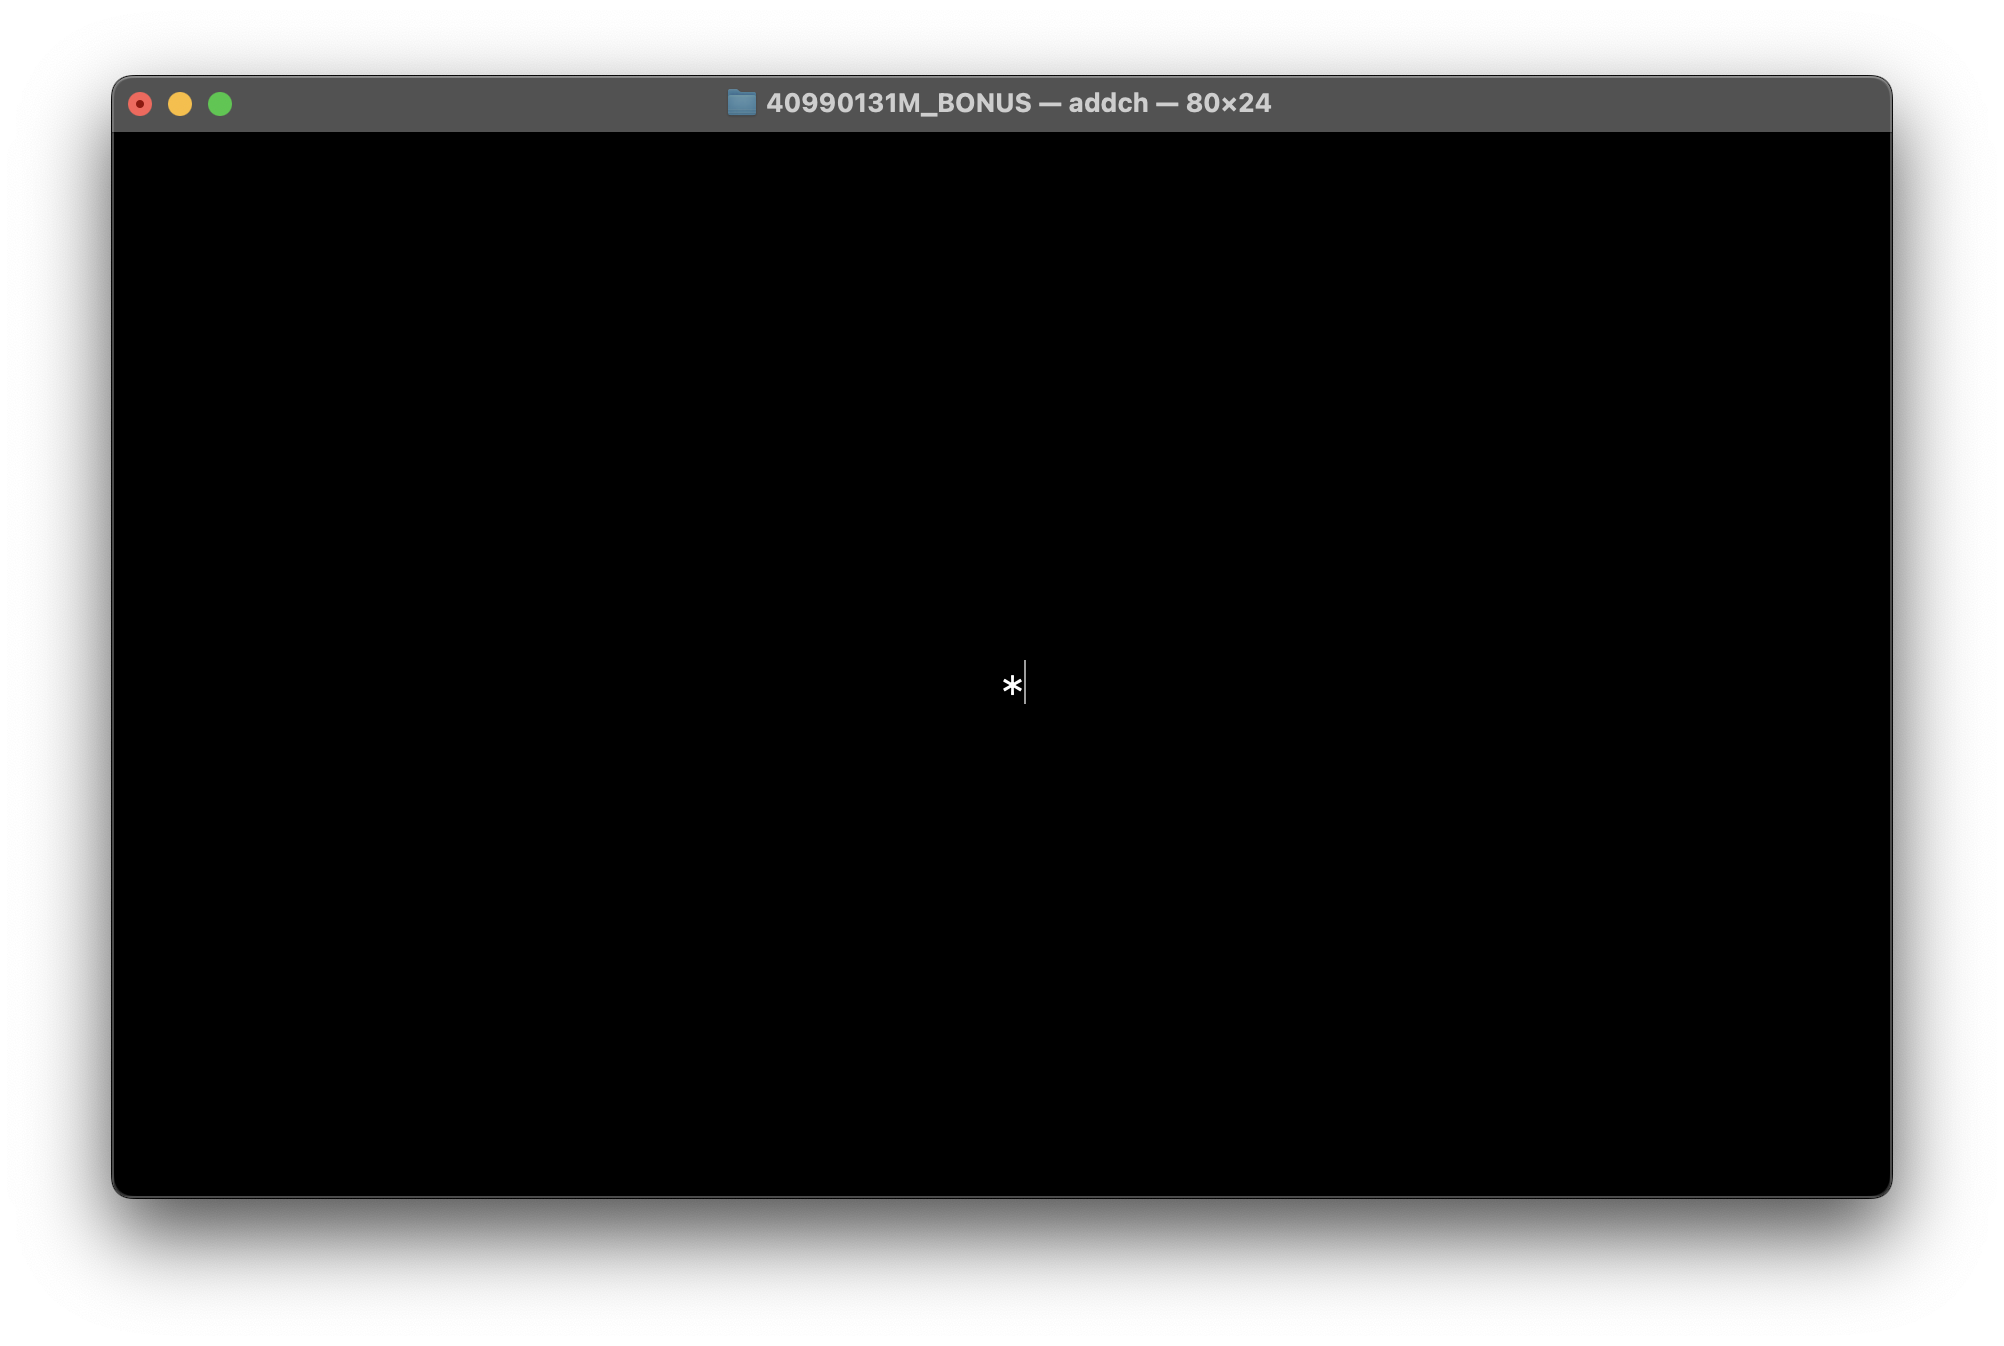
\includegraphics[width=\textwidth]{addch.png}
\end{center}
另外,第 11-12 行可以合併為以下形式:
\begin{lstlisting}[style=C*]
  mvaddch(12, 40, '*');
\end{lstlisting}
另外,注意上述的 \texttt{addch()} 與 \texttt{mvaddch()} 是輸出到視窗 \texttt{stdscr} 上,如果要輸出到其它視窗,必須使用 \texttt{waddch()} 與 \texttt{mvwaddch()} 函式。

\subsubsection{\texttt{printw()}}
\noindent
\hypertarget{2.2.2}{以下程式展示}
了 \texttt{mvprintw()} 函式的使用方法:
\begin{lstlisting}[style=C]
  // printw.c
  #include <string.h>
  #include <ncurses.h>

  int main()
  {
      initscr();
      raw();
      noecho();
    
      int row = 0, col = 0;
      getmaxyx(stdscr, row, col); // 取得視窗大小資訊
      char message[] = "Hello world!";
      // 移動 cursor 並將 message 印在視窗中央
      mvprintw(row/2, (col-strlen(message))/2, "%s", message);
    
      refresh();
      getch();
      endwin();
      return 0;
  }
\end{lstlisting}
執行結果如下:
\begin{lstlisting}[style=zsh]
  % ./printw
\end{lstlisting}
\begin{center}
    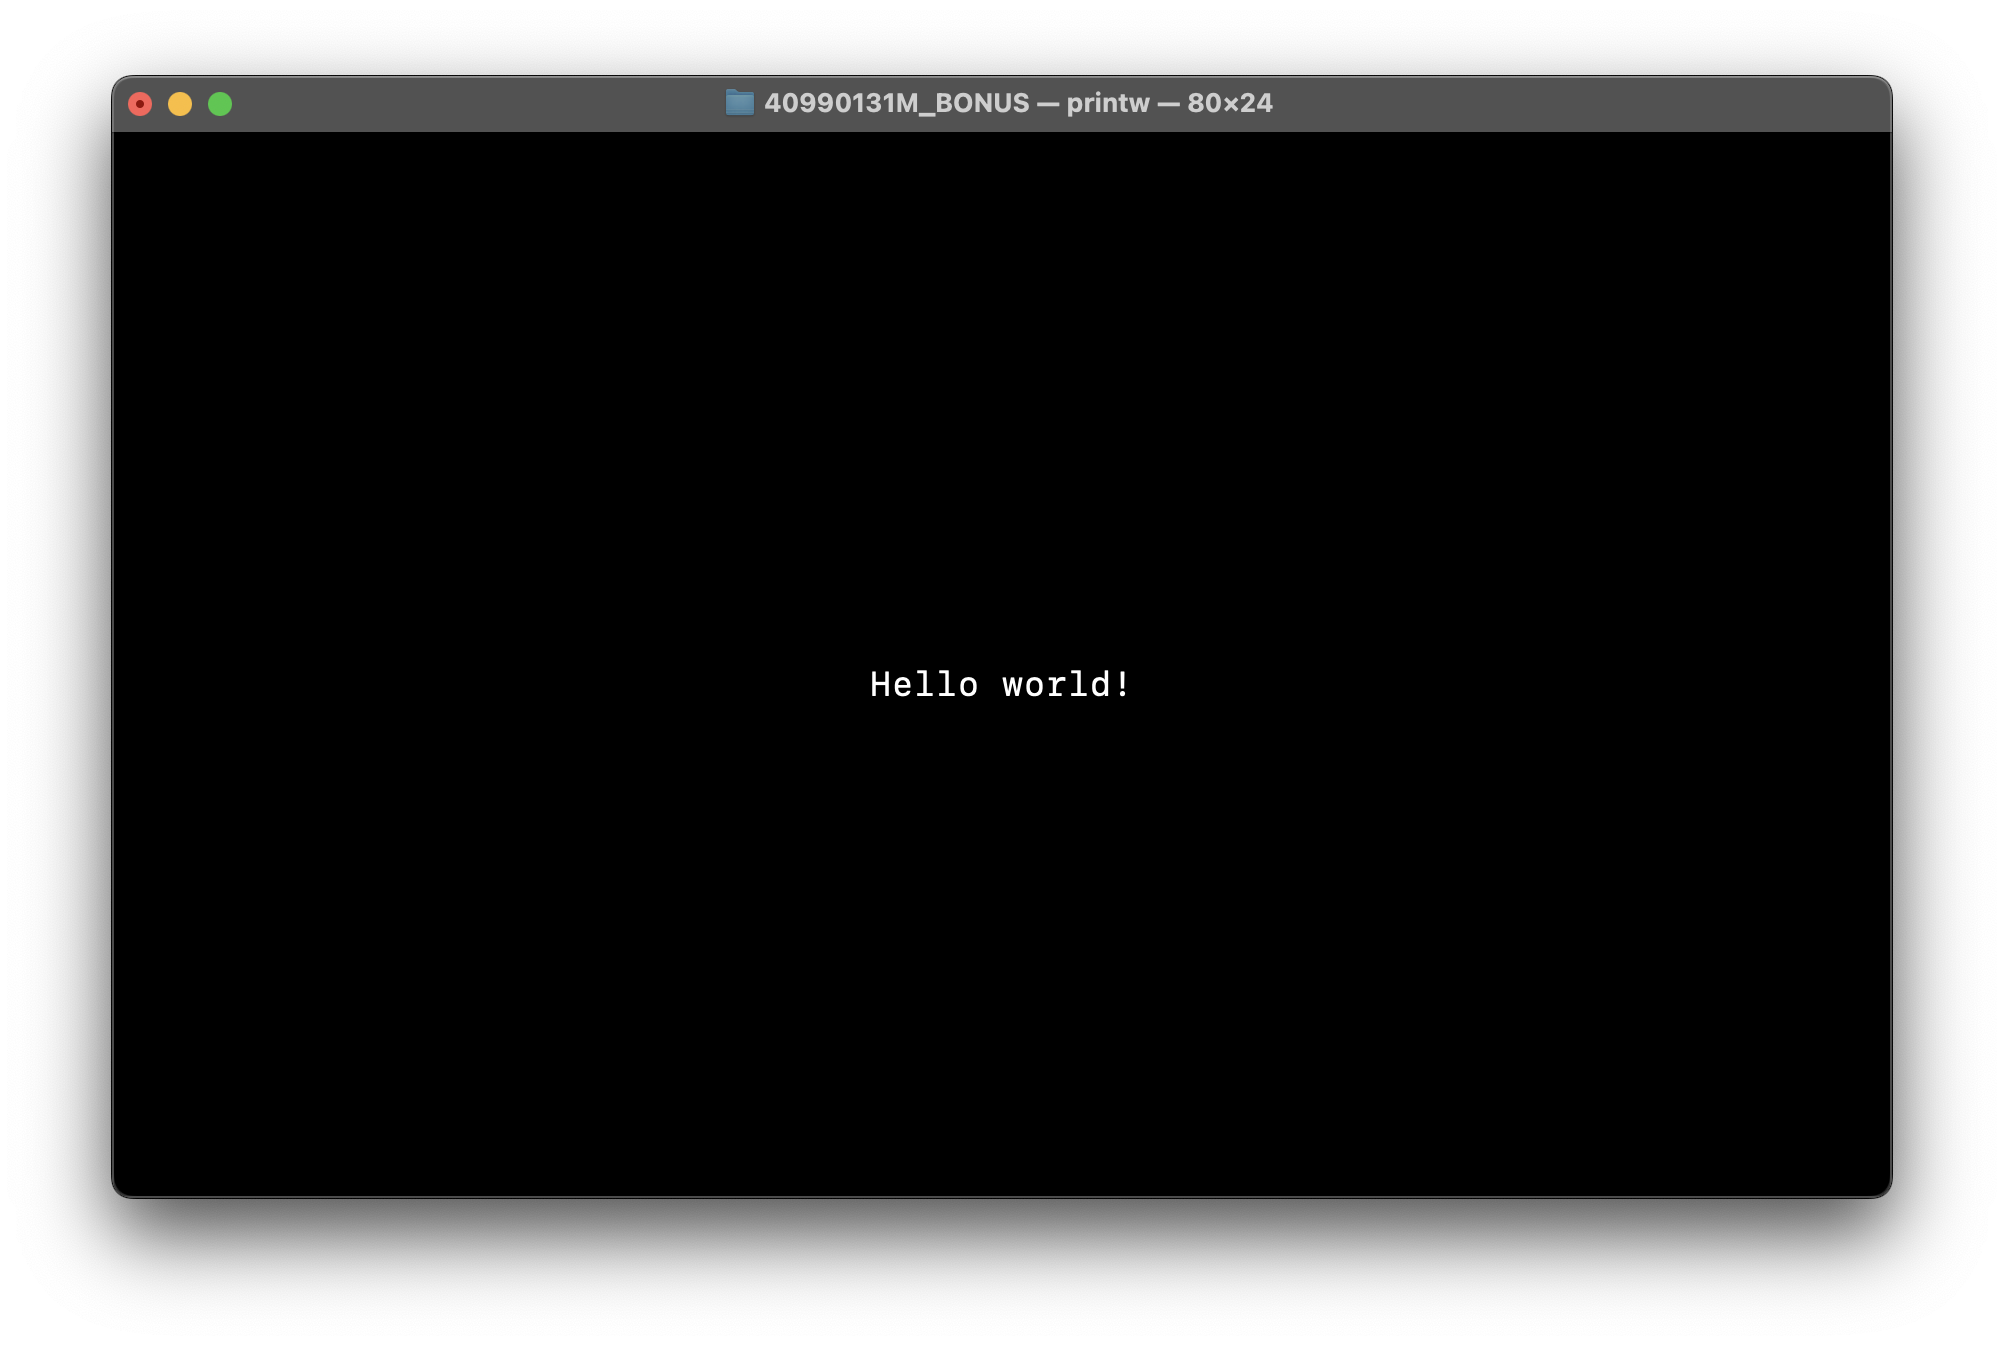
\includegraphics[width=\linewidth]{printw.png}
\end{center}
以上的函式中的 \texttt{mvprintw()} 與以下效果相當:
\begin{lstlisting}[style=C*]
  move(row/2, (col-strlen(message))/2);
  printw("%s", message);
\end{lstlisting}
與 \texttt{mvaddch()} 類似,\texttt{printw()} 與 \texttt{mvprintw()} 也是輸出到視窗 \texttt{stdscr} 上,如果要輸出到其它視窗,\hypertarget{2.2.2a}{必須使用} \texttt{wprintw()} 與 \texttt{mvwprintw()} 函式。另外,有一個函式 \texttt{vwprintw()} 與 \texttt{vprintf()} 有著對應的功能,可以印出 variable length of argument 的 formatted string。

\subsubsection{\texttt{addstr()}}
\noindent
\hypertarget{2.2.3}{另外一個種類的輸出相關函式}可以被視為 \texttt{addch()} 函式家族的 string 版本。我們這次嘗試在不同位置印出 Hello world 訊息:
\begin{lstlisting}[style=C]
  // addstr.c
  #include <ncurses.h>

  int main()
  {
      initscr();
      raw();
      noecho();
    
      mvaddstr(12, 0, "Hello world!");
    
      refresh();
      getch();
      endwin();
      return 0;
  }
\end{lstlisting}
以上的程式與上一節中的執行結果一致,如下圖:
\begin{lstlisting}[style=zsh]
  % ./addstr
\end{lstlisting}
\begin{center}
    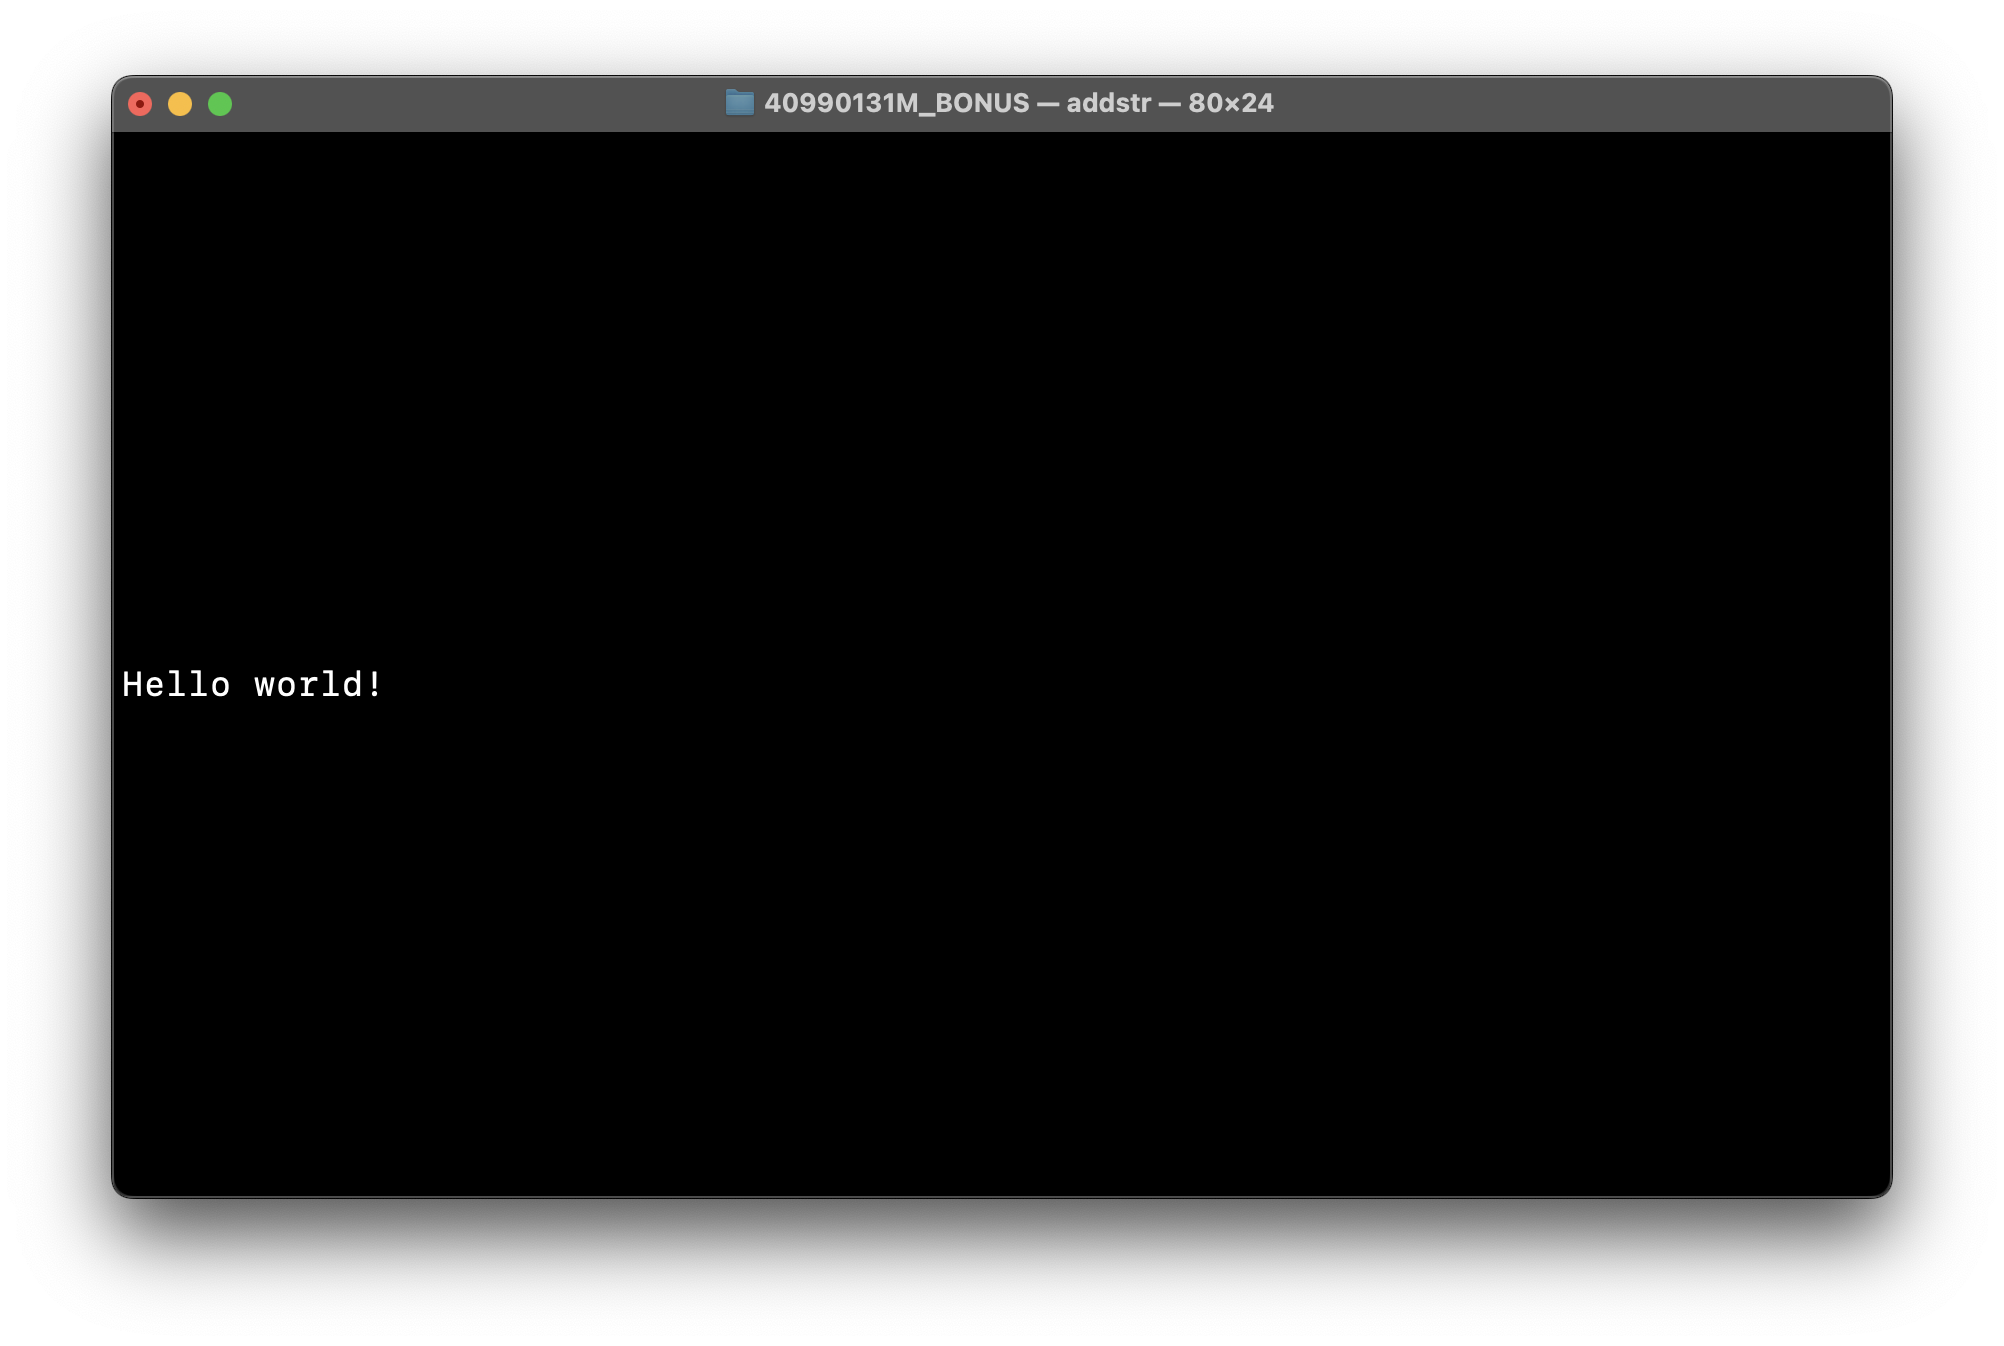
\includegraphics[width=\linewidth]{addstr.png}
\end{center}
如果要輸出到不同視窗,必須用 \texttt{waddstr()} 或 \texttt{mvwaddstr()} 函式。另外,函式 \texttt{addnstr()} 可以限制印出的字數不超過 $n$ 個,如果 $n<0$ 則字串會被完整地顯示。

\subsubsection{\texttt{getmaxyx()}}
\noindent
在 \hyperlink{2.2.2}{2.2.2} 與 \hyperlink{2.2.3}{2.2.3} 中,我們使用 \texttt{getmaxyx()} 來取得視窗的大小資訊,以將資訊印在視窗中央。不過,\texttt{getmaxyx()} 其實是一個定義在 \texttt{ncurses.h} 中的 macro,因此在使用上我們會代入兩個型別為 \texttt{int} 的變數。注意在每一個函式中,$y$座標皆在$x$座標的前面。

\subsubsection{\texttt{getch()}}
\noindent
從上一個章節開始,\texttt{getch()} 就出現在每一個範例程式中,擔任等待使用者輸入的角色。在之前的程式中,使用者輸入後即馬上執行下一個 \texttt{endwin()} 函式結束 \texttt{ncurses} 模式。而在接下來的範例程式中,我們會讓使用者輸入一個字符 (chracter) 並印出使用者輸入的字符:
\begin{lstlisting}[style=C]
  // getch.c
  #include <string.h>
  #include <ncurses.h>

  int main()
  {
      initscr();
      cbreak();
      noecho();
    
      printw("Enter a character: ");
      int ch = getch();
      printw("\nYou entered '%c'\n", ch);
    
      refresh();
      getch();
      endwin();
      return 0;
  }
\end{lstlisting}
注意,此處我們用 \texttt{cbreak()} 取代了 \texttt{raw()},兩者的作用相似但有一些差異。與輸出的函式相似,與 \texttt{getch()} 用法相似的還有 \texttt{mvgetch()}、\texttt{wgetch()} 與 \texttt{mvwgetch()} 函式。

\subsubsection{\texttt{scanw()}}
與 \texttt{scanw()} 有關的函式包含 \texttt{mvscanw()}、\texttt{wscanw()}、\texttt{mvwscanw()}、\texttt{vscanw()},其使用方法與 \texttt{printw()} 相似,不在此贅述。

\subsubsection{\texttt{getstr()}}
與 \texttt{getstr()} 有關的函式包含 \texttt{mvgetstr()}、\texttt{wgetstr()}、\texttt{mvwgetstr()}、\texttt{getnstr()}、\texttt{mvgetnstr()}、\texttt{wgetnstr()}、\texttt{mvwgetnstr()},這些函式的命名方法與前相同,因此不在此多加描述。

\subsection{屬性}
\noindent
我們用以下範例程式來說明屬性的運用:
\begin{lstlisting}[style=C]
  // attribute.c
  #include <string.h>
  #include <ncurses.h>

  int main()
  {
      initscr();
      cbreak();
      noecho();
    
      attron(A_BOLD);         // Enable the Bold Attribute
      mvprintw(4, 8, "1");
      attron(A_UNDERLINE);    // Enable the Underlining Attribute
      mvprintw(8, 4, "2");
      attroff(A_BOLD);        // Disable the Bold Attribute
      mvprintw(12, 0, "3");
      attrset(A_REVERSE);     // Set to Reverse Attribute
      mvprintw(16, 12, "4");
      attrset(A_NORMAL);      // Set to Normal Attribute
      mvprintw(20, 0, "5");
    
      refresh();
      getch();
      endwin();
      return 0;
  }
\end{lstlisting}
注意其中的 \texttt{attron()} 與 \texttt{attroff()} 只會更動指定的屬性,而 \texttt{attrset()} 會將視窗設置只開啟指定的屬性。實際效果如下:
\begin{lstlisting}[style=zsh]
  % ./attribute
\end{lstlisting}
\begin{center}
    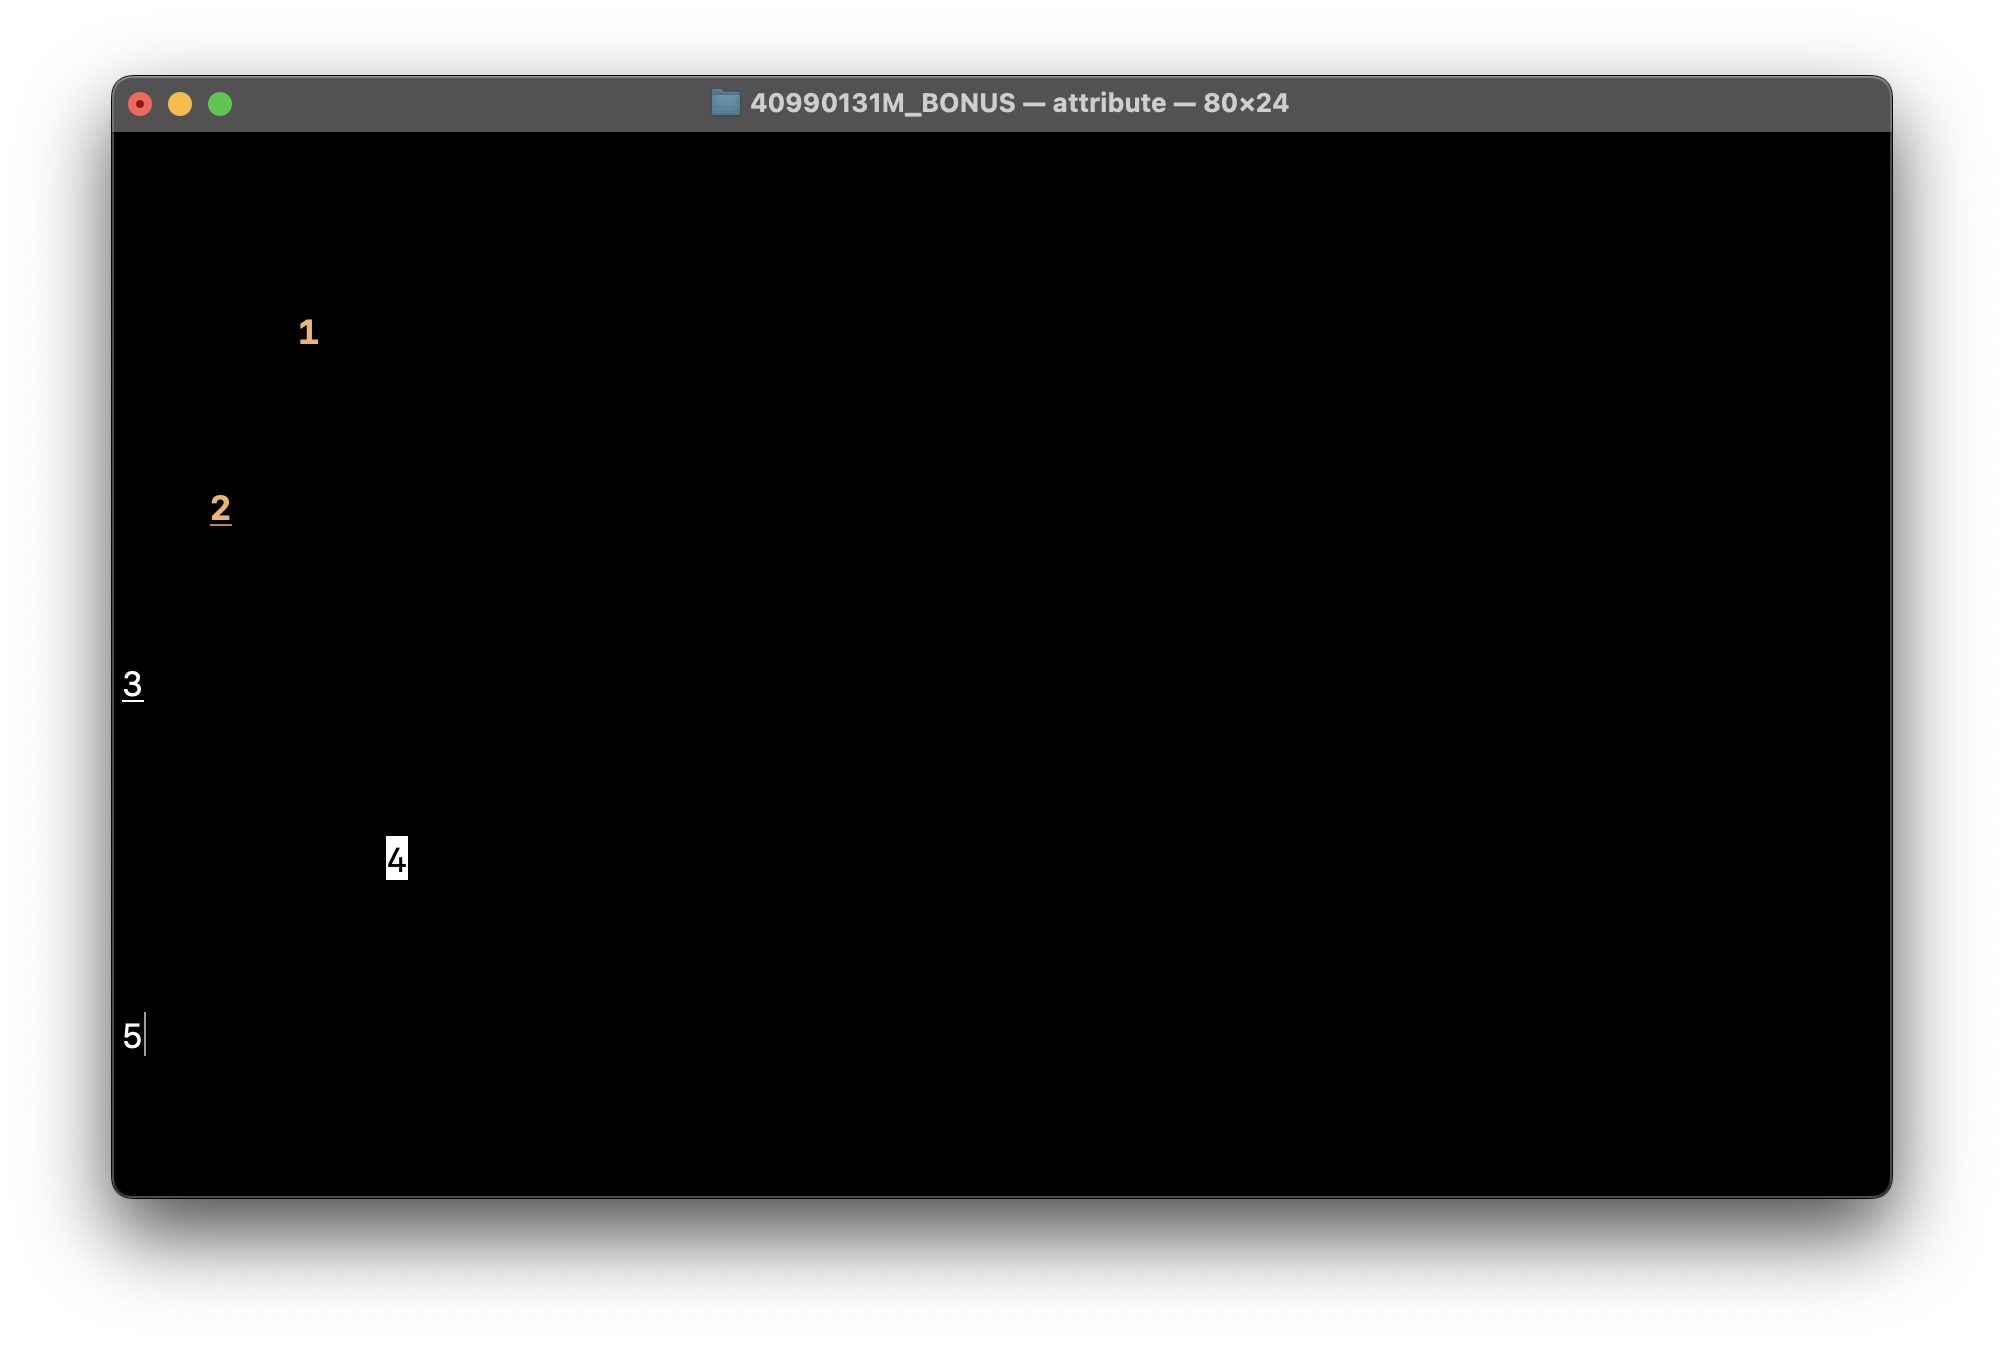
\includegraphics[width=\textwidth]{attribute.png}
\end{center}

\subsubsection{色彩}
\noindent
在屬性中,有一個重要的屬性是色彩。在以下的範例程式中,我們展示如何使用色彩:
\begin{lstlisting}[style=C]
  // color.c
  #include <stdlib.h>
  #include <ncurses.h>

  int main()
  {
      initscr();
      cbreak();
      noecho();
    
      // Check if the terminal support color
      if (has_colors() == FALSE)
      {
          endwin();
          printf("Your terminal does not support color.\n");
          exit(1);
      }
    
      // Initialize color settings
      start_color();
      init_pair(1, COLOR_RED, COLOR_YELLOW);
      init_pair(2, COLOR_GREEN, COLOR_BLUE);
    
      int row = 0, col = 0, diag = 0;
      getmaxyx(stdscr, row, col);
      diag = (row < col) ? row : col;
    
      for (int i = 0; i < diag; i++)
      {
          attron(COLOR_PAIR(i % 3));
          mvaddch(i, i, '*');
          attroff(COLOR_PAIR(i % 3));
      }
    
      refresh();
      getch();
      endwin();
      return 0;
  }
\end{lstlisting}
以下為執行結果:
\begin{lstlisting}[style=zsh]
  % ./color
\end{lstlisting}
\begin{center}
    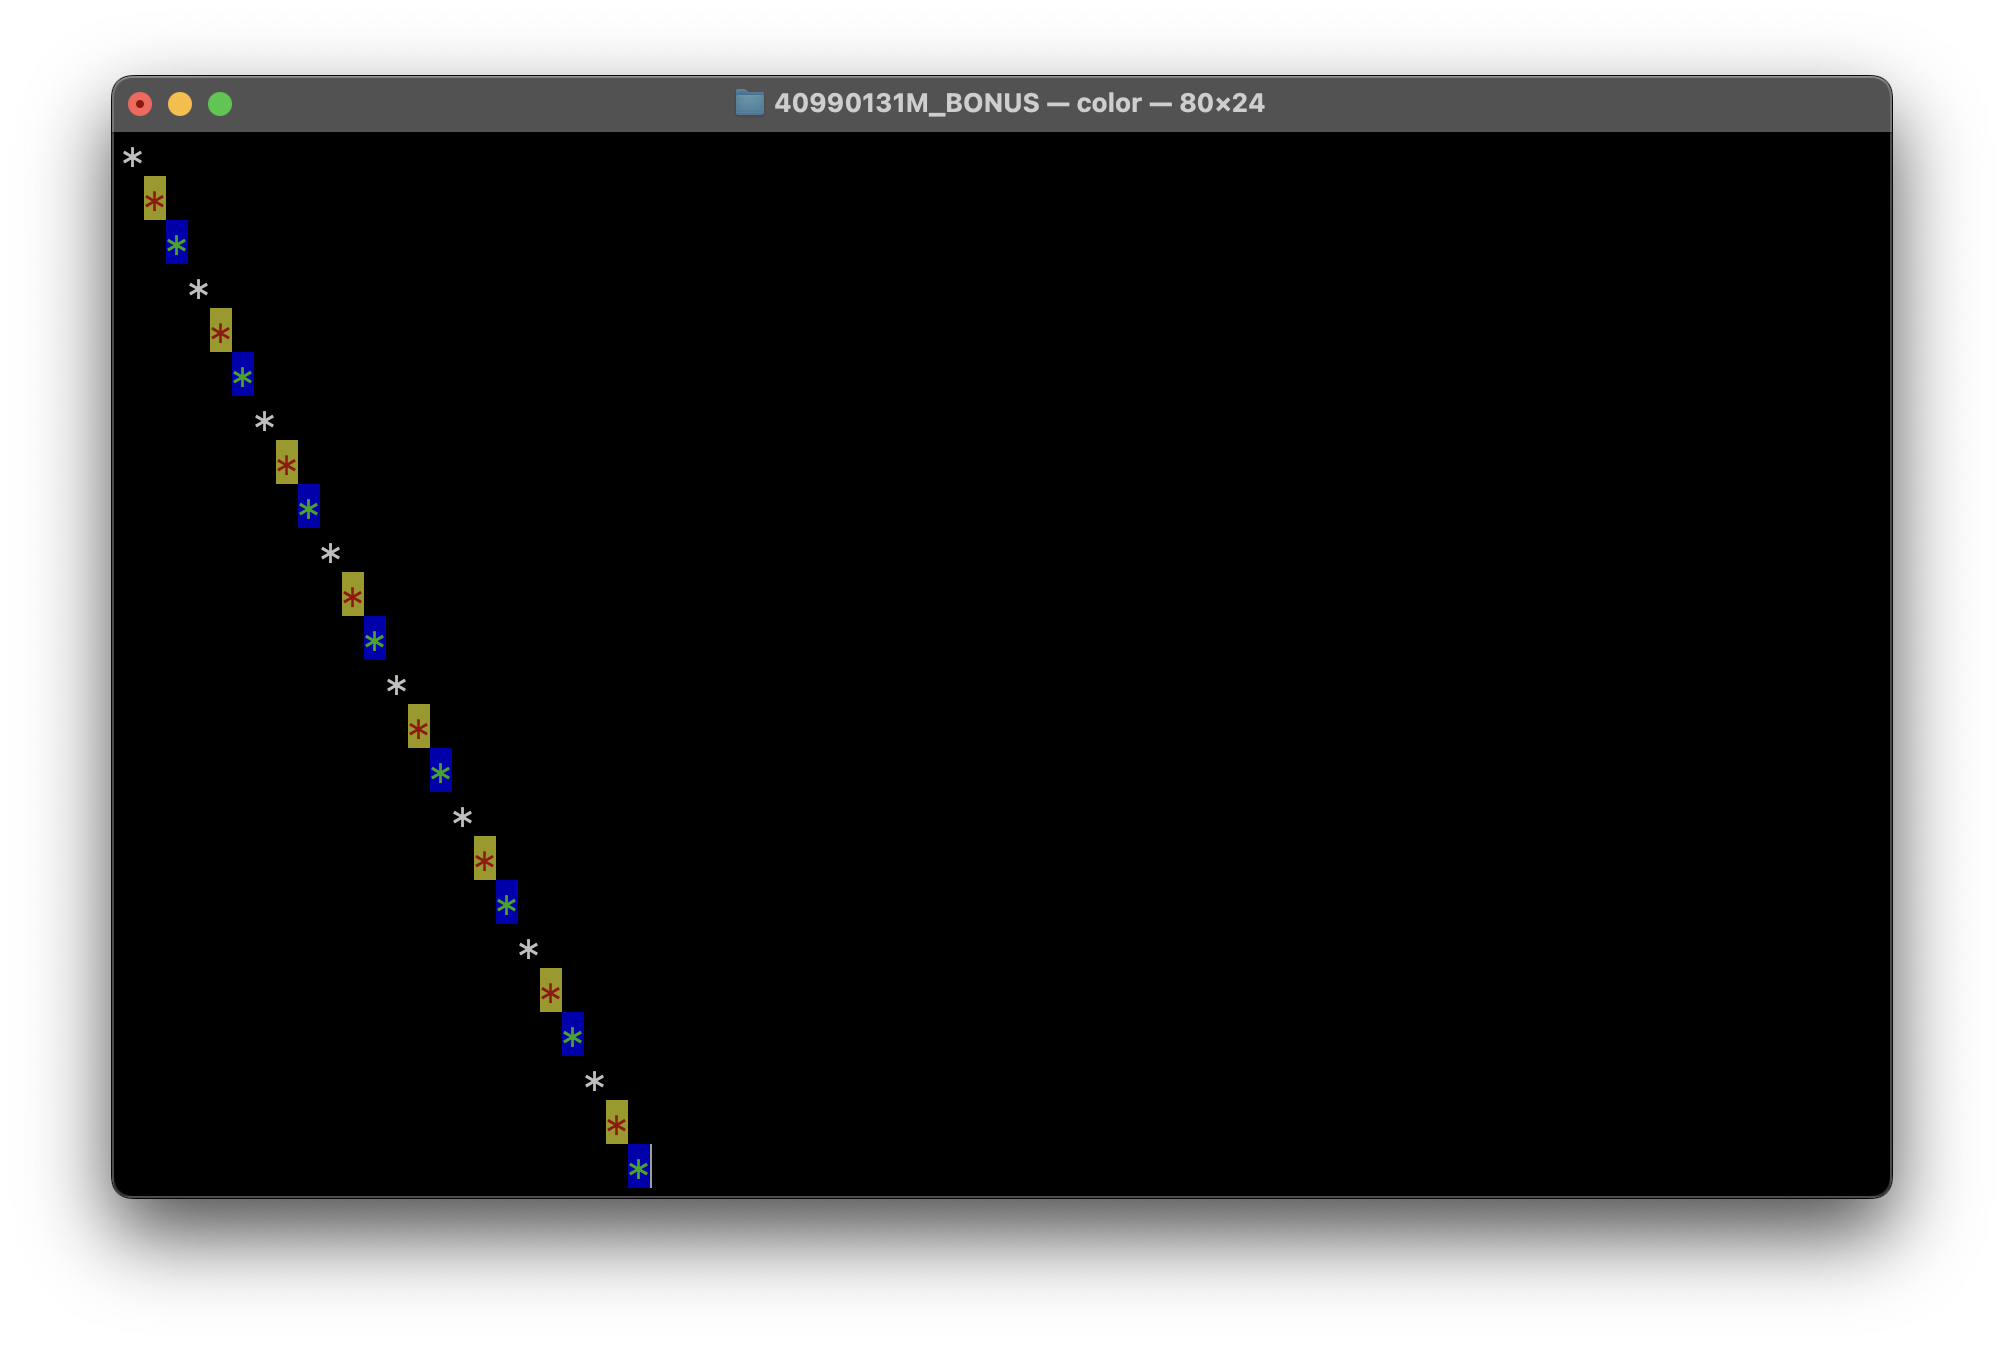
\includegraphics[width=\textwidth]{color.png}
\end{center}

\subsection{視窗}
\noindent
使用 \texttt{ncurses} 最重要的其中一件事情就是創造許多不同的視窗,並且適當地操縱這些視窗是相當重要的。以下的範例程式簡單展示了視窗的基本操作:
\begin{lstlisting}[style=C]
  // window.c
  #include <ncurses.h>

  int main()
  {
      initscr();
      cbreak();
      noecho();
    
      WINDOW *myWin = newwin(10, 30, 5, 10);  // Create a new window
      box(myWin, 0, 0);                       // Draw border

      mvwprintw(myWin, 1, 1, "This is myWin!");
      refresh();
      wrefresh(myWin);

      getch();
      delwin(myWindow);  // Delete the window
      endwin();
      return 0;
  }
\end{lstlisting}
第 10 行的 \texttt{newwin(10, 30, 5, 10)} 創造了一個從第 10 列到第 30 列、從第 5 行到第 10 行的視窗,而 \texttt{box()} 為視窗 \texttt{myWin} 創造了邊界。我們在 \hyperlink{2.2.2a}{2.2.2} 中提過,\texttt{mvwprintw()} 可用於對 \texttt{stdscr} 以外的視窗進行 \texttt{mvprintw()}。而第 15 行的 \texttt{wrefresh()} 函式的命名也是相似的邏輯。一般的 \texttt{refresh()} 函式更新的是 \texttt{stdscr} 視窗,而 \texttt{wrefresh()} 則可以用於指定的視窗。上述程式執行的結果如下:
\begin{lstlisting}[style=zsh]
  % ./window
\end{lstlisting}
\begin{center}
    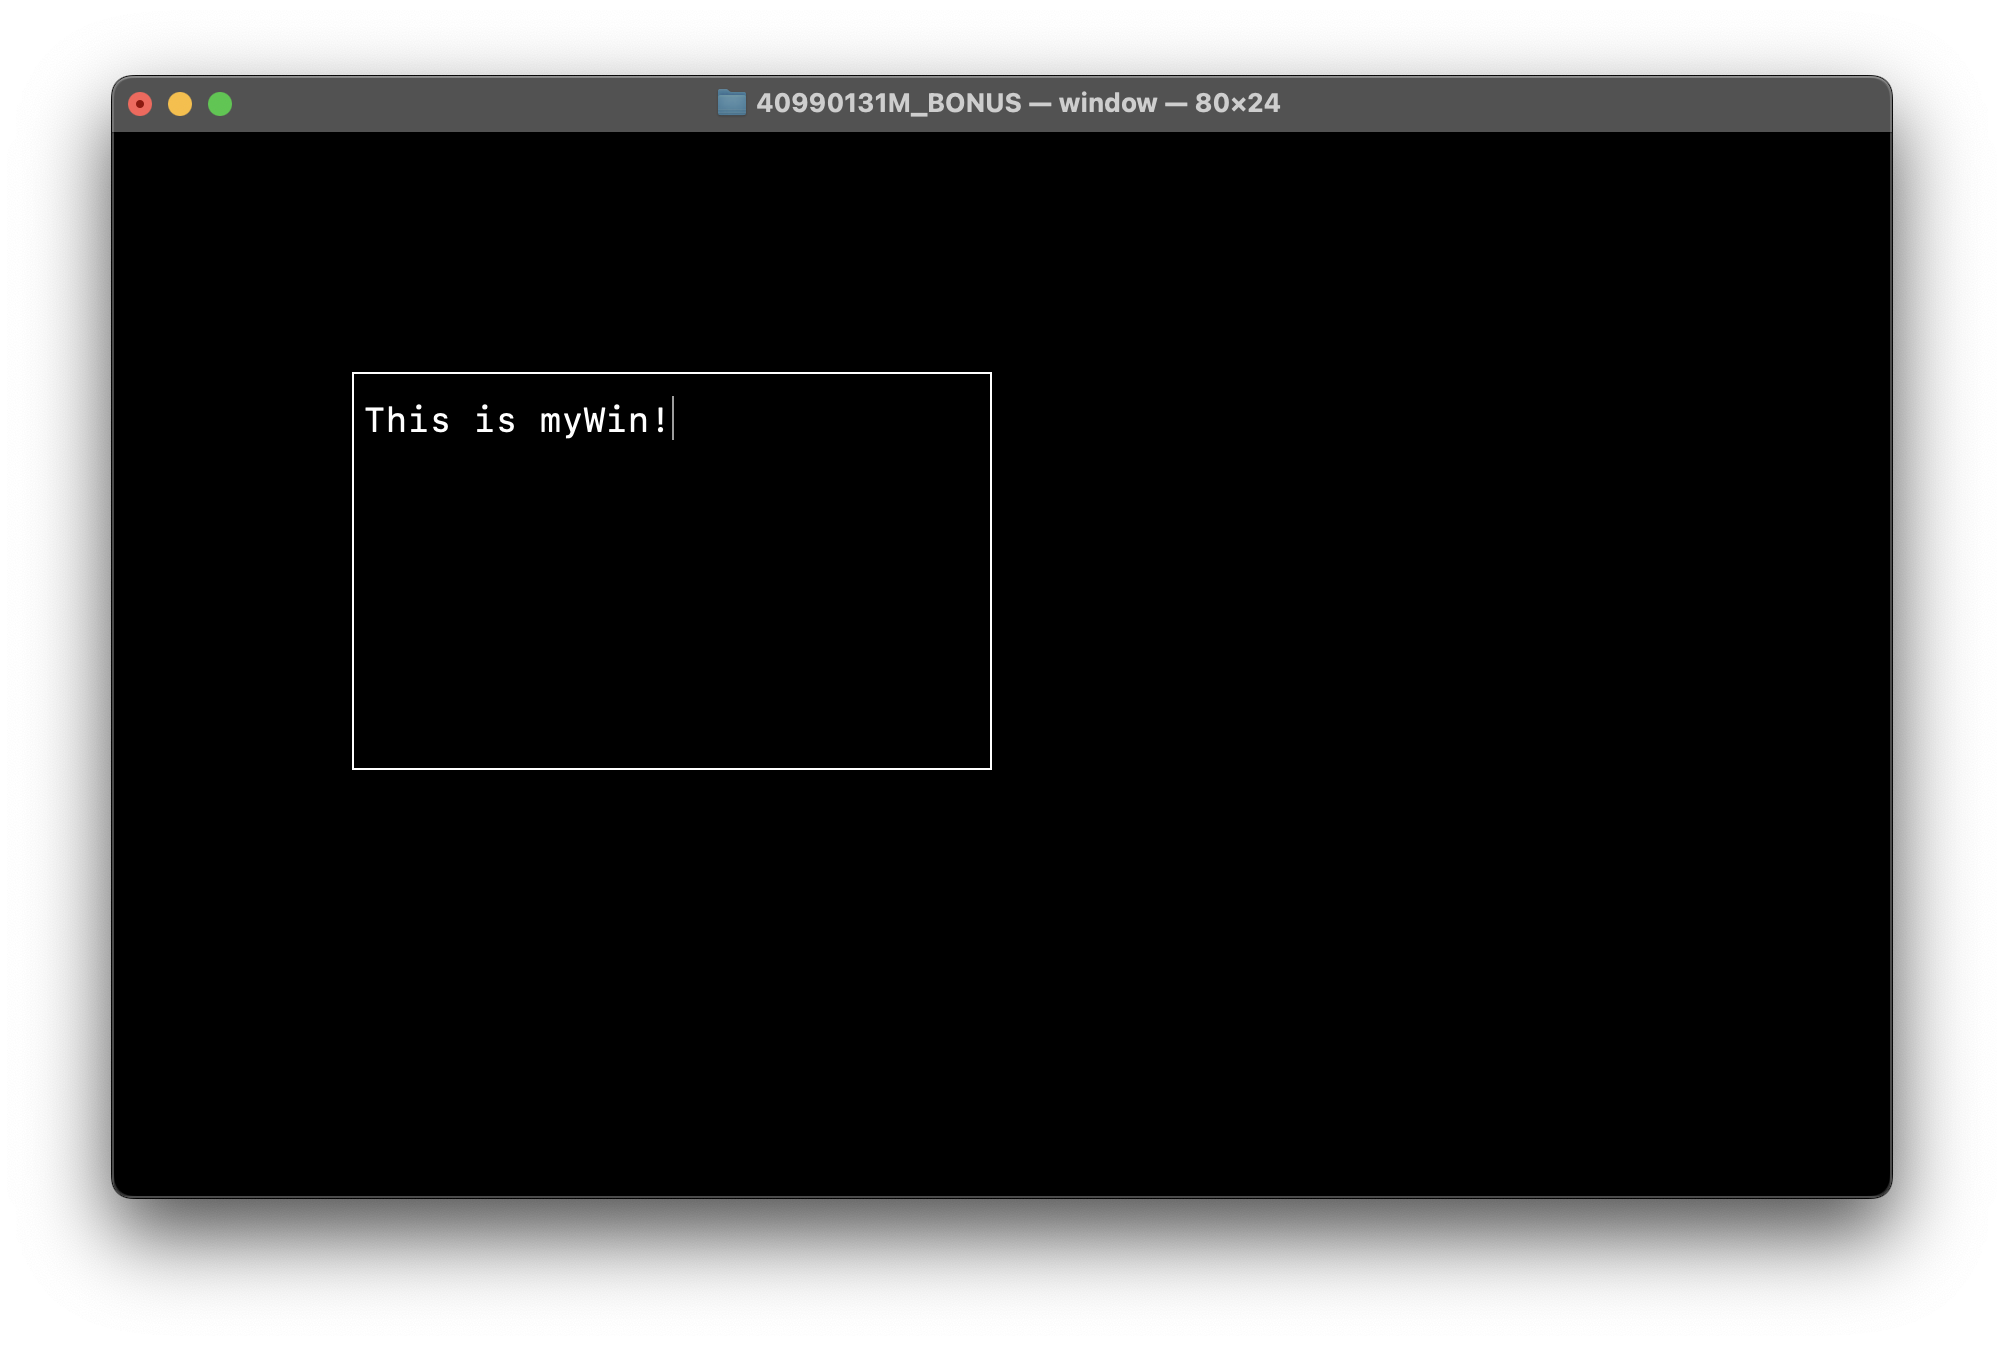
\includegraphics[width=\textwidth]{window.png}
\end{center}

\subsection{鍵盤介面}
\noindent
在與使用者互動的過程中,收集鍵盤與滑鼠資訊是很重要的事。以下這個範例程式呈現鍵盤的偵測:
\begin{lstlisting}[style=C]
  // keyboard.c
  #include <ncurses.h>

  int main()
  {
      initscr();
      cbreak();
      noecho();
    
      keypad(stdscr, TRUE);  // 啟用偵測按鍵
      mvprintw(1, 0, "Press the arrow keys. Press 'q' to quit.");
      move(3, 0);
    
      int ch = 0;
      while ((ch = getch()) != 'q')
      {
          switch (ch)
          {
              case KEY_LEFT:
                  printw("Left arrow key is pressed.\n");
                  break;
              case KEY_RIGHT:
                  printw("Right arrow key is pressed.\n");
                  break;
              case KEY_UP:
                  printw("Up arrow key is pressed.\n");
                  break;
              case KEY_DOWN:
                  printw("Down arrow key is pressed.\n");
                  break;
              default:
                  printw("Unknown key is pressed.\n");
                  break;
          }
          refresh();
      }
    
      endwin();
      return 0;
  }
\end{lstlisting}
執行的結果如下
\begin{lstlisting}[style=zsh]
  % ./keyboard
\end{lstlisting}
\begin{center}
    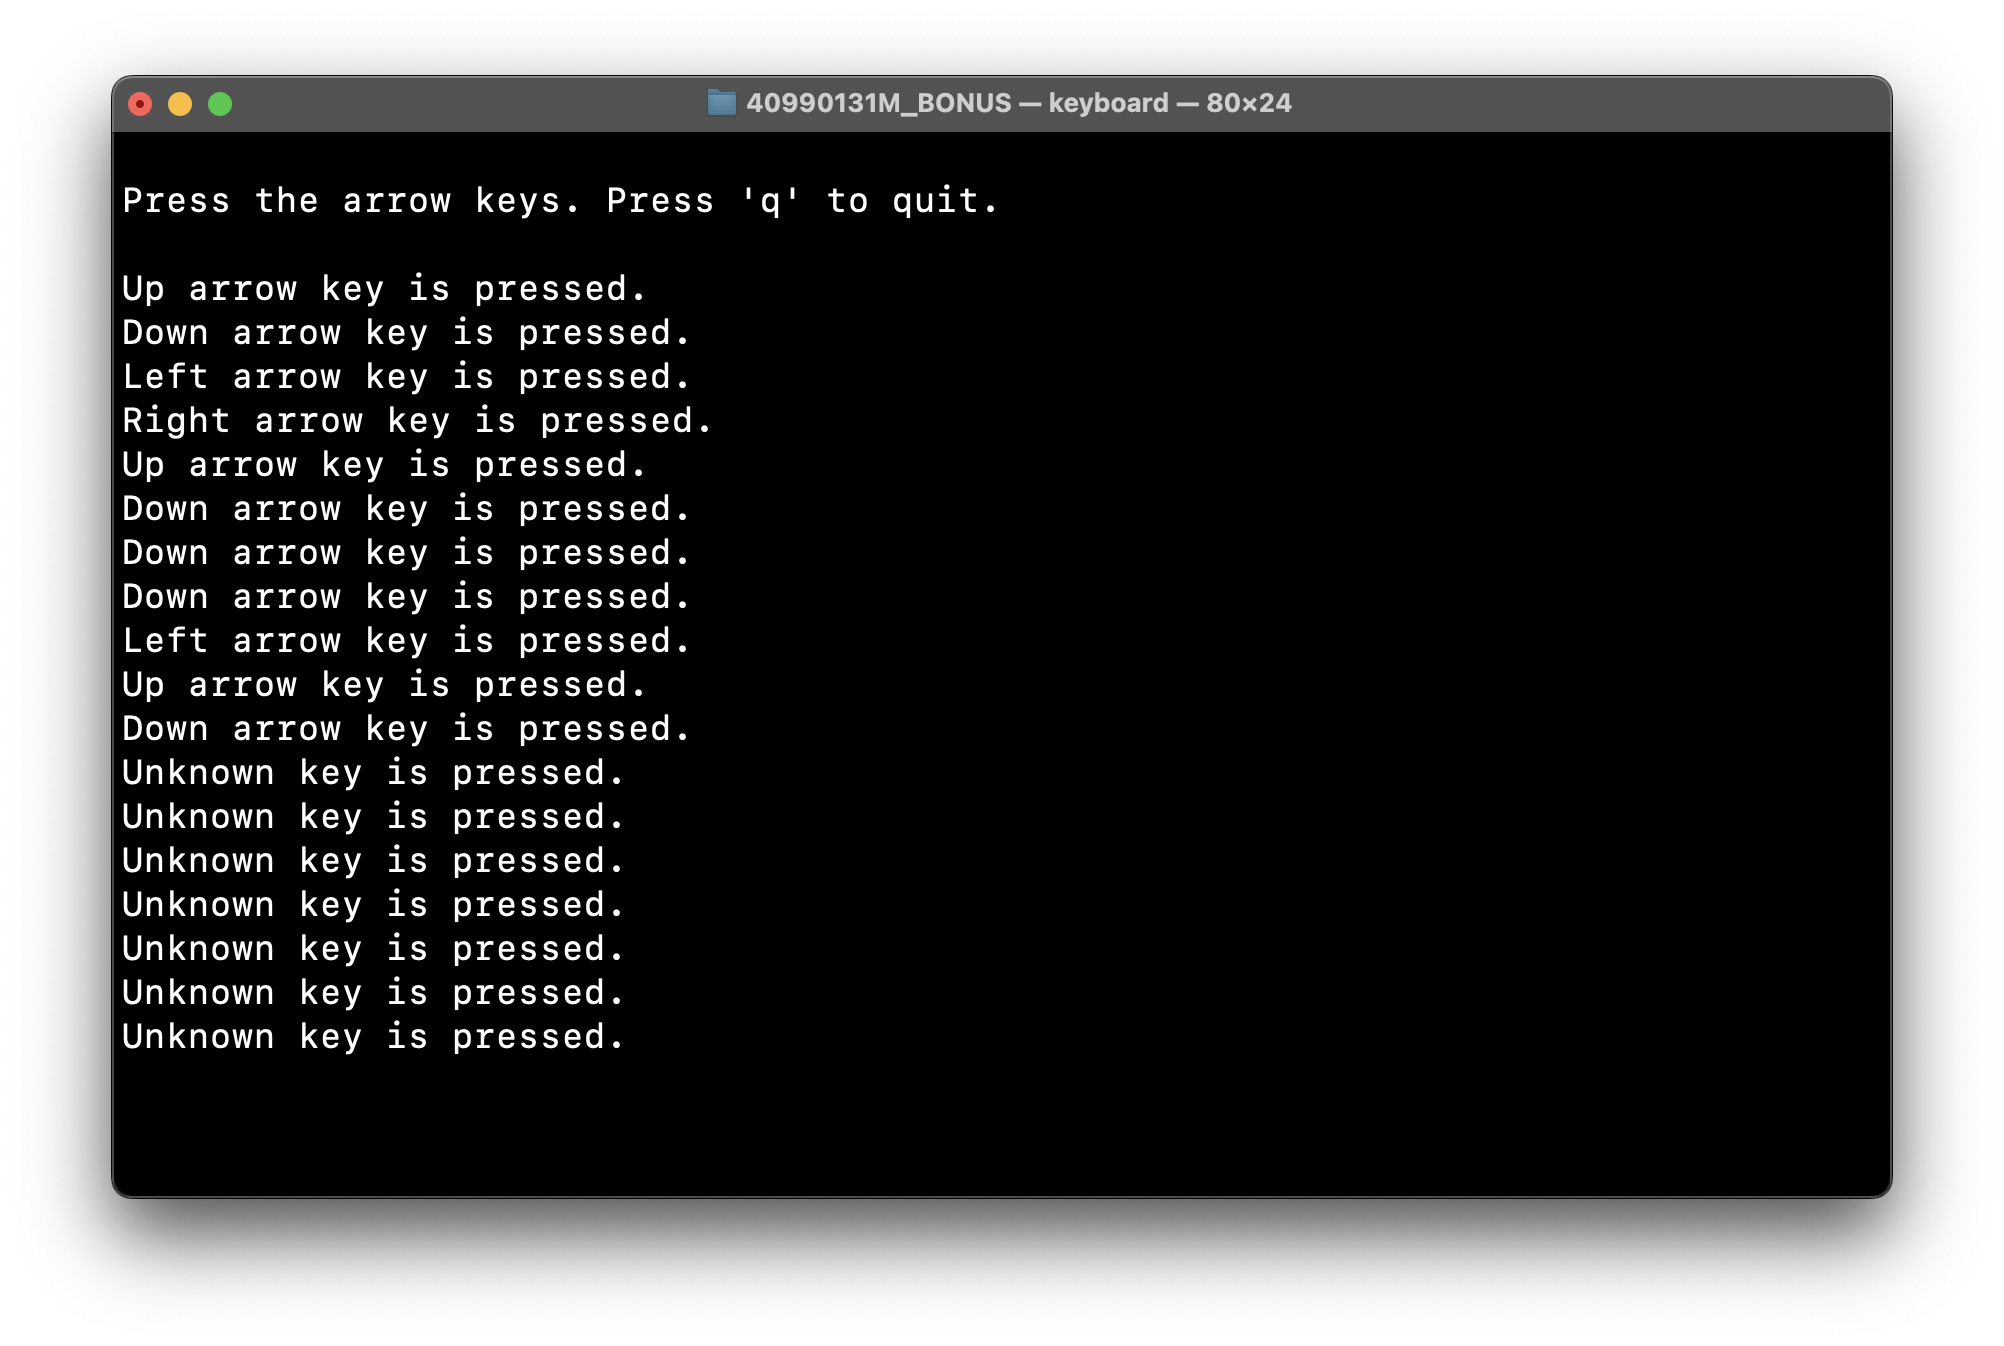
\includegraphics[width=\textwidth]{keyboard.png}
\end{center}

\newpage
\noindent
另外,我們也可以啟用 mouse events,函式 \texttt{getch()} 此時會返回 \texttt{KEY\_MOUSE} 並且可以使用函式 \texttt{getmouse()} 來得到事件的資訊。因為較為複雜且非必要,因此在此不涵蓋滑鼠相關的內容。

\nocite{ncurses-howto}
\printbibliography
\end{document}